\documentclass{standalone}
\usepackage{tikz}
\usetikzlibrary{patterns, positioning}
\usepackage[sfdefault]{ClearSans} %% option 'sfdefault' activates Clear Sans as the default text font
\usepackage[T1]{fontenc}

\begin{document}
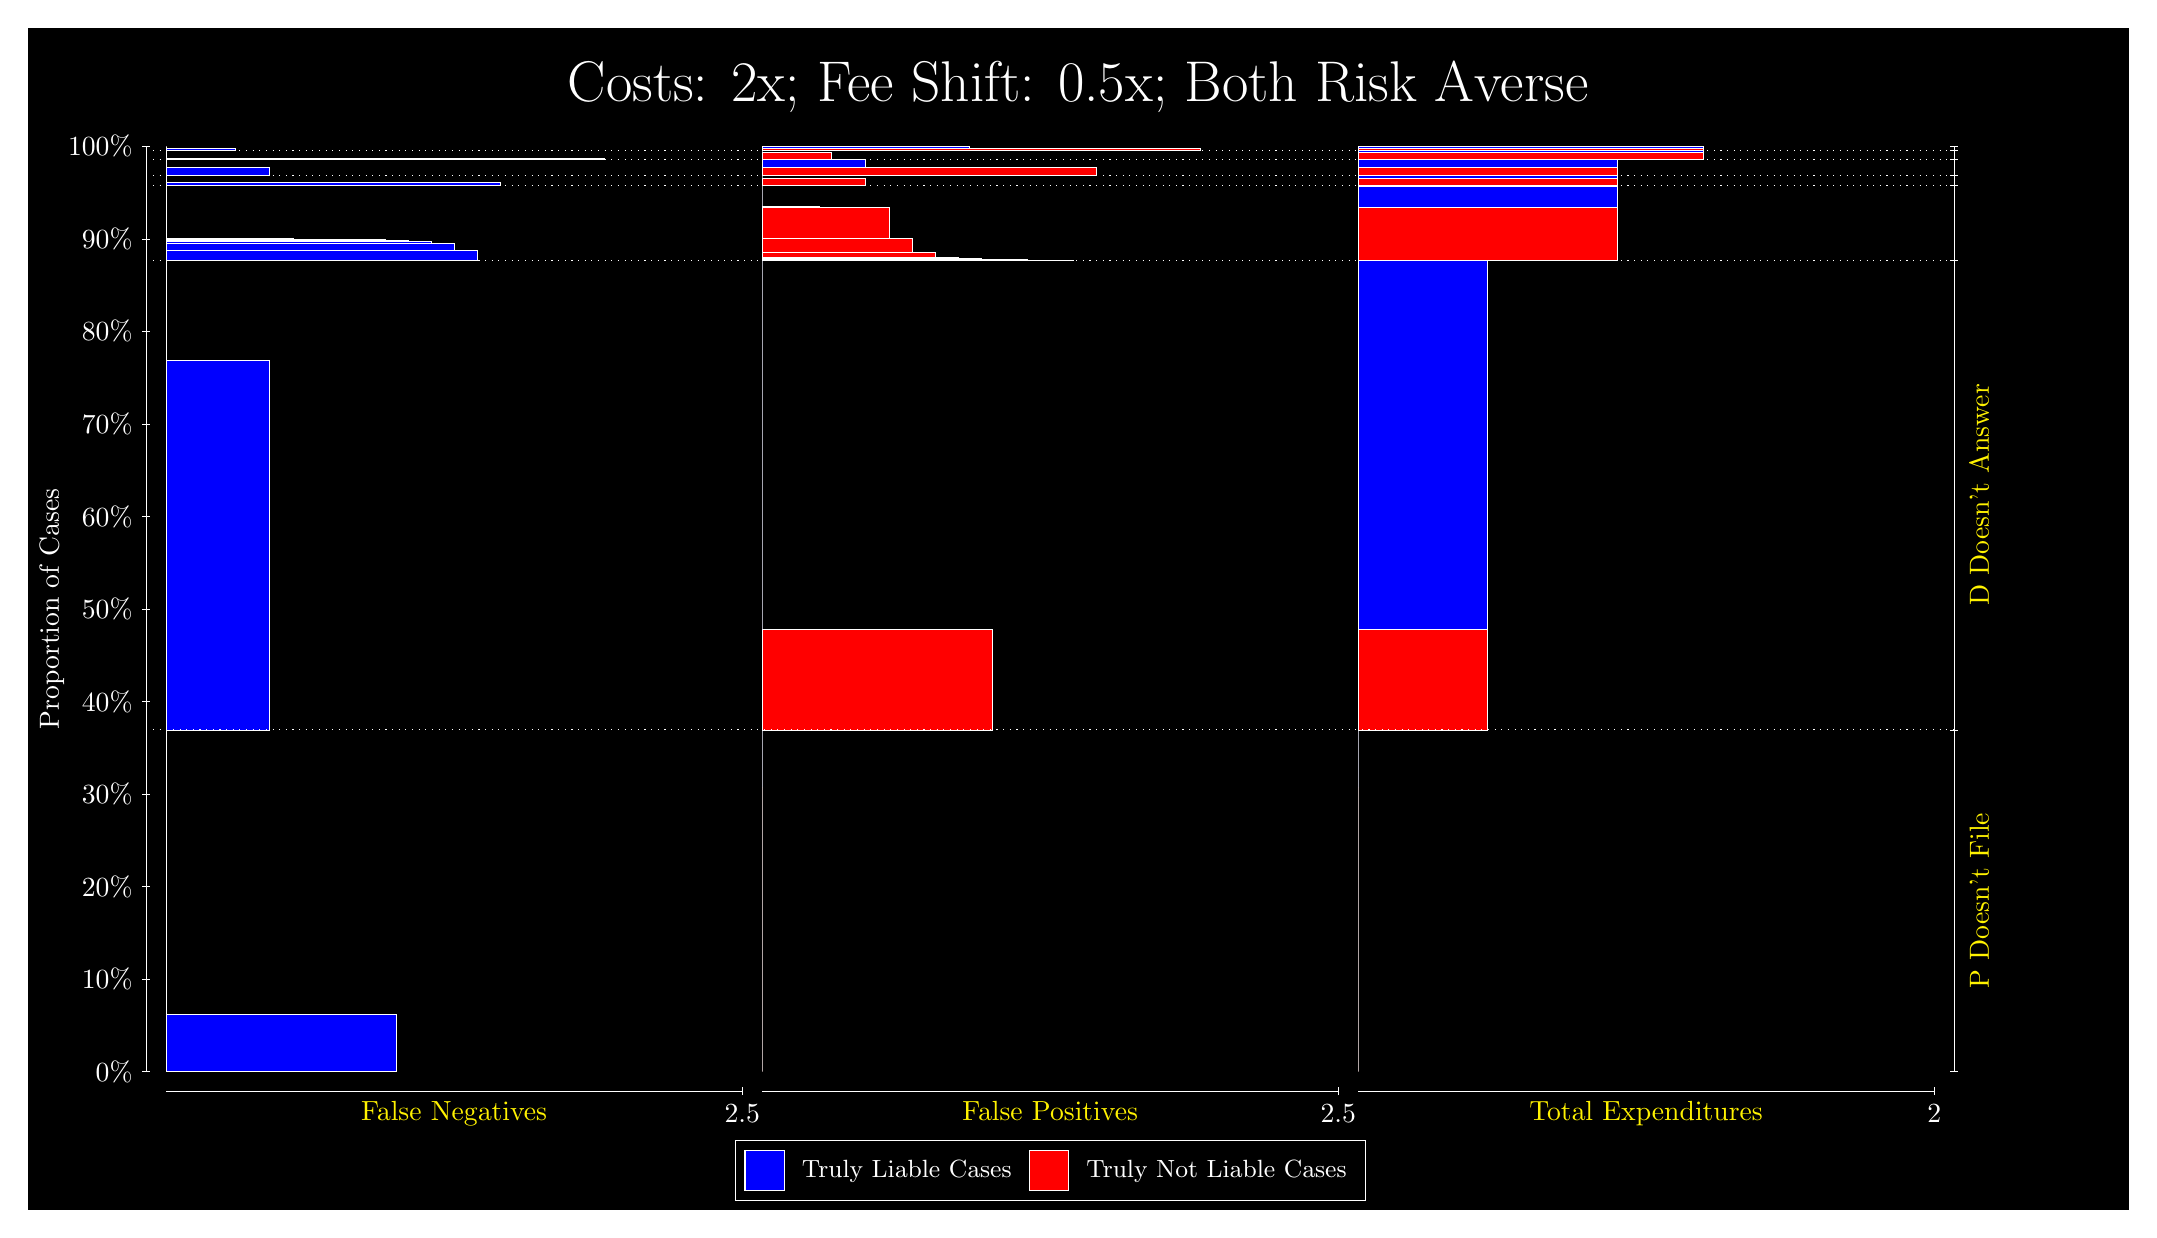
\begin{tikzpicture}
\draw[fill=black] (0,0) rectangle (26.667,15);
\draw[text=white] (0,13.5) rectangle (26.667,15) node[midway] {\huge Costs: 2x; Fee Shift: 0.5x; Both Risk Averse};
\draw[white, very thin] (1.5,1.75) -- (1.5,13.5);
\node[rotate=90, text=white, anchor=center] at (0.3, 7.625) {Proportion of Cases};
\draw[white, very thin] (1.45,1.75) -- (1.55,1.75);
\node[text=white, anchor=east] at (1.45, 1.75) {0\%};
\draw[white, very thin] (1.45,2.925) -- (1.55,2.925);
\node[text=white, anchor=east] at (1.45, 2.925) {10\%};
\draw[white, very thin] (1.45,4.1) -- (1.55,4.1);
\node[text=white, anchor=east] at (1.45, 4.1) {20\%};
\draw[white, very thin] (1.45,5.275) -- (1.55,5.275);
\node[text=white, anchor=east] at (1.45, 5.275) {30\%};
\draw[white, very thin] (1.45,6.45) -- (1.55,6.45);
\node[text=white, anchor=east] at (1.45, 6.45) {40\%};
\draw[white, very thin] (1.45,7.625) -- (1.55,7.625);
\node[text=white, anchor=east] at (1.45, 7.625) {50\%};
\draw[white, very thin] (1.45,8.8) -- (1.55,8.8);
\node[text=white, anchor=east] at (1.45, 8.8) {60\%};
\draw[white, very thin] (1.45,9.975) -- (1.55,9.975);
\node[text=white, anchor=east] at (1.45, 9.975) {70\%};
\draw[white, very thin] (1.45,11.15) -- (1.55,11.15);
\node[text=white, anchor=east] at (1.45, 11.15) {80\%};
\draw[white, very thin] (1.45,12.325) -- (1.55,12.325);
\node[text=white, anchor=east] at (1.45, 12.325) {90\%};
\draw[white, very thin] (1.45,13.5) -- (1.55,13.5);
\node[text=white, anchor=east] at (1.45, 13.5) {100\%};

\draw[white, very thin] (24.457,1.75) -- (24.457,13.5);
\draw[white, very thin] (24.407,1.75) -- (24.507,1.75);
\node[anchor=west] at (24.407, 1.75) {};
\draw[white, very thin] (24.407,6.0894) -- (24.507,6.0894);
\node[anchor=west] at (24.407, 6.0894) {};
\draw[white, very thin] (24.407,12.055) -- (24.507,12.055);
\node[anchor=west] at (24.407, 12.055) {};
\draw[white, very thin] (24.407,13.001) -- (24.507,13.001);
\node[anchor=west] at (24.407, 13.001) {};
\draw[white, very thin] (24.407,13.135) -- (24.507,13.135);
\node[anchor=west] at (24.407, 13.135) {};
\draw[white, very thin] (24.407,13.332) -- (24.507,13.332);
\node[anchor=west] at (24.407, 13.332) {};
\draw[white, very thin] (24.407,13.451) -- (24.507,13.451);
\node[anchor=west] at (24.407, 13.451) {};
\draw[white, very thin] (24.407,13.5) -- (24.507,13.5);
\node[anchor=west] at (24.407, 13.5) {};

\draw[white, very thin, fill=blue] (1.75,1.75) rectangle (4.6775,2.4775);
\draw[white, very thin, fill=red] (1.75,2.4775) rectangle (1.75,6.0894);
\draw[white, very thin, fill=blue] (1.75,6.0894) rectangle (3.0674,10.782);
\draw[white, very thin, fill=red] (1.75,10.782) rectangle (1.75,12.055);
\draw[white, very thin, fill=blue] (1.75,12.055) rectangle (5.7022,12.181);
\draw[white, very thin, fill=blue] (1.75,12.181) rectangle (5.4094,12.266);
\draw[white, very thin, fill=blue] (1.75,12.266) rectangle (5.1167,12.295);
\draw[white, very thin, fill=blue] (1.75,12.295) rectangle (4.8239,12.303);
\draw[white, very thin, fill=blue] (1.75,12.303) rectangle (4.8239,12.305);
\draw[white, very thin, fill=blue] (1.75,12.305) rectangle (4.5312,12.314);
\draw[white, very thin, fill=blue] (1.75,12.314) rectangle (4.2384,12.317);
\draw[white, very thin, fill=blue] (1.75,12.317) rectangle (3.9457,12.321);
\draw[white, very thin, fill=blue] (1.75,12.321) rectangle (3.6529,12.324);
\draw[white, very thin, fill=blue] (1.75,12.324) rectangle (3.3602,12.326);
\draw[white, very thin, fill=red] (1.75,12.326) rectangle (1.75,13.001);
\draw[white, very thin, fill=blue] (1.75,13.001) rectangle (5.9949,13.041);
\draw[white, very thin, fill=red] (1.75,13.041) rectangle (1.75,13.135);
\draw[white, very thin, fill=blue] (1.75,13.135) rectangle (3.0674,13.23);
\draw[white, very thin, fill=red] (1.75,13.23) rectangle (1.75,13.332);
\draw[white, very thin, fill=blue] (1.75,13.332) rectangle (7.3123,13.354);
\draw[white, very thin, fill=red] (1.75,13.354) rectangle (1.75,13.451);
\draw[white, very thin, fill=blue] (1.75,13.451) rectangle (2.6283,13.479);
\draw[white, very thin, fill=red] (1.75,13.479) rectangle (1.75,13.5);
\draw[white, very thin, fill=red] (9.3189,1.75) rectangle (9.3189,5.3619);
\draw[white, very thin, fill=blue] (9.3189,5.3619) rectangle (9.3189,6.0894);
\draw[white, very thin, fill=red] (9.3189,6.0894) rectangle (12.246,7.3628);
\draw[white, very thin, fill=blue] (9.3189,7.3628) rectangle (9.3189,12.055);
\draw[white, very thin, fill=red] (9.3189,12.055) rectangle (13.271,12.056);
\draw[white, very thin, fill=red] (9.3189,12.056) rectangle (12.978,12.058);
\draw[white, very thin, fill=red] (9.3189,12.058) rectangle (12.686,12.061);
\draw[white, very thin, fill=red] (9.3189,12.061) rectangle (12.393,12.065);
\draw[white, very thin, fill=red] (9.3189,12.065) rectangle (12.1,12.078);
\draw[white, very thin, fill=red] (9.3189,12.078) rectangle (11.807,12.081);
\draw[white, very thin, fill=red] (9.3189,12.081) rectangle (11.807,12.093);
\draw[white, very thin, fill=red] (9.3189,12.093) rectangle (11.515,12.15);
\draw[white, very thin, fill=red] (9.3189,12.15) rectangle (11.222,12.338);
\draw[white, very thin, fill=red] (9.3189,12.338) rectangle (10.929,12.73);
\draw[white, very thin, fill=blue] (9.3189,12.73) rectangle (10.344,12.731);
\draw[white, very thin, fill=blue] (9.3189,12.731) rectangle (10.051,12.734);
\draw[white, very thin, fill=blue] (9.3189,12.734) rectangle (9.758,12.739);
\draw[white, very thin, fill=blue] (9.3189,12.739) rectangle (9.4652,12.742);
\draw[white, very thin, fill=blue] (9.3189,12.742) rectangle (9.3189,13.001);
\draw[white, very thin, fill=red] (9.3189,13.001) rectangle (10.636,13.095);
\draw[white, very thin, fill=blue] (9.3189,13.095) rectangle (9.3189,13.135);
\draw[white, very thin, fill=red] (9.3189,13.135) rectangle (13.564,13.238);
\draw[white, very thin, fill=blue] (9.3189,13.238) rectangle (10.636,13.332);
\draw[white, very thin, fill=red] (9.3189,13.332) rectangle (10.197,13.43);
\draw[white, very thin, fill=blue] (9.3189,13.43) rectangle (9.3189,13.451);
\draw[white, very thin, fill=red] (9.3189,13.451) rectangle (14.881,13.473);
\draw[white, very thin, fill=blue] (9.3189,13.473) rectangle (11.954,13.5);
\draw[white, very thin, fill=red] (16.888,1.75) rectangle (16.888,5.3619);
\draw[white, very thin, fill=blue] (16.888,5.3619) rectangle (16.888,6.0894);
\draw[white, very thin, fill=red] (16.888,6.0894) rectangle (18.534,7.3628);
\draw[white, very thin, fill=blue] (16.888,7.3628) rectangle (18.534,12.055);
\draw[white, very thin, fill=red] (16.888,12.055) rectangle (20.181,12.056);
\draw[white, very thin, fill=blue] (16.888,12.056) rectangle (20.181,12.058);
\draw[white, very thin, fill=red] (16.888,12.058) rectangle (20.181,12.728);
\draw[white, very thin, fill=blue] (16.888,12.728) rectangle (20.181,12.994);
\draw[white, very thin, fill=red] (16.888,12.994) rectangle (20.181,12.998);
\draw[white, very thin, fill=blue] (16.888,12.998) rectangle (20.181,13.001);
\draw[white, very thin, fill=red] (16.888,13.001) rectangle (20.181,13.095);
\draw[white, very thin, fill=blue] (16.888,13.095) rectangle (20.181,13.135);
\draw[white, very thin, fill=red] (16.888,13.135) rectangle (20.181,13.238);
\draw[white, very thin, fill=blue] (16.888,13.238) rectangle (20.181,13.332);
\draw[white, very thin, fill=red] (16.888,13.332) rectangle (21.279,13.43);
\draw[white, very thin, fill=blue] (16.888,13.43) rectangle (21.279,13.451);
\draw[white, very thin, fill=red] (16.888,13.451) rectangle (21.279,13.473);
\draw[white, very thin, fill=blue] (16.888,13.473) rectangle (21.279,13.5);
\draw[white, dotted] (1.5,6.0894) -- (24.457,6.0894);
\draw[white, dotted] (1.5,12.055) -- (24.457,12.055);
\draw[white, dotted] (1.5,13.001) -- (24.457,13.001);
\draw[white, dotted] (1.5,13.135) -- (24.457,13.135);
\draw[white, dotted] (1.5,13.332) -- (24.457,13.332);
\draw[white, dotted] (1.5,13.451) -- (24.457,13.451);
\draw[white, very thin] (1.75,1.5) -- (9.0689,1.5);
\node[text=yellow, anchor=north] at (5.4094, 1.5) {False Negatives};
\draw[white, very thin] (9.0689,1.45) -- (9.0689,1.55);
\node[text=white, anchor=north] at (9.0689, 1.45) {2.5};

\draw[white, very thin] (9.3189,1.5) -- (16.638,1.5);
\node[text=yellow, anchor=north] at (12.978, 1.5) {False Positives};
\draw[white, very thin] (16.638,1.45) -- (16.638,1.55);
\node[text=white, anchor=north] at (16.638, 1.45) {2.5};

\draw[white, very thin] (16.888,1.5) -- (24.207,1.5);
\node[text=yellow, anchor=north] at (20.547, 1.5) {Total Expenditures};
\draw[white, very thin] (24.207,1.45) -- (24.207,1.55);
\node[text=white, anchor=north] at (24.207, 1.45) {2};

\node[text=yellow, centered, rotate=90] at (24.777, 3.9197) {P Doesn't File};
\node[text=yellow, centered, rotate=90] at (24.777, 9.0722) {D Doesn't Answer};






\draw (12.978300999999998,1.5) node[draw=none] (baseCoordinate) {};
\begin{scope}[align=center]
        \matrix[scale=0.5, draw=white, below=0.5cm of baseCoordinate, nodes={draw}, column sep=0.1cm]{
            \node[rectangle, draw, minimum width=0.5cm, minimum height=0.5cm, fill=blue] {}; &
            \node[draw=none, font=\small, text=white] (B) {Truly Liable Cases}; &
            \node[rectangle, draw, minimum width=0.5cm, minimum height=0.5cm, fill=red] {}; &
            \node[draw=none, font=\small, text=white] (B) {Truly Not Liable Cases}; \\
            };
\end{scope}

\end{tikzpicture}
\end{document}